	\section{Historie}
\label{sec:history}

\begin{frame}{\TeX}
  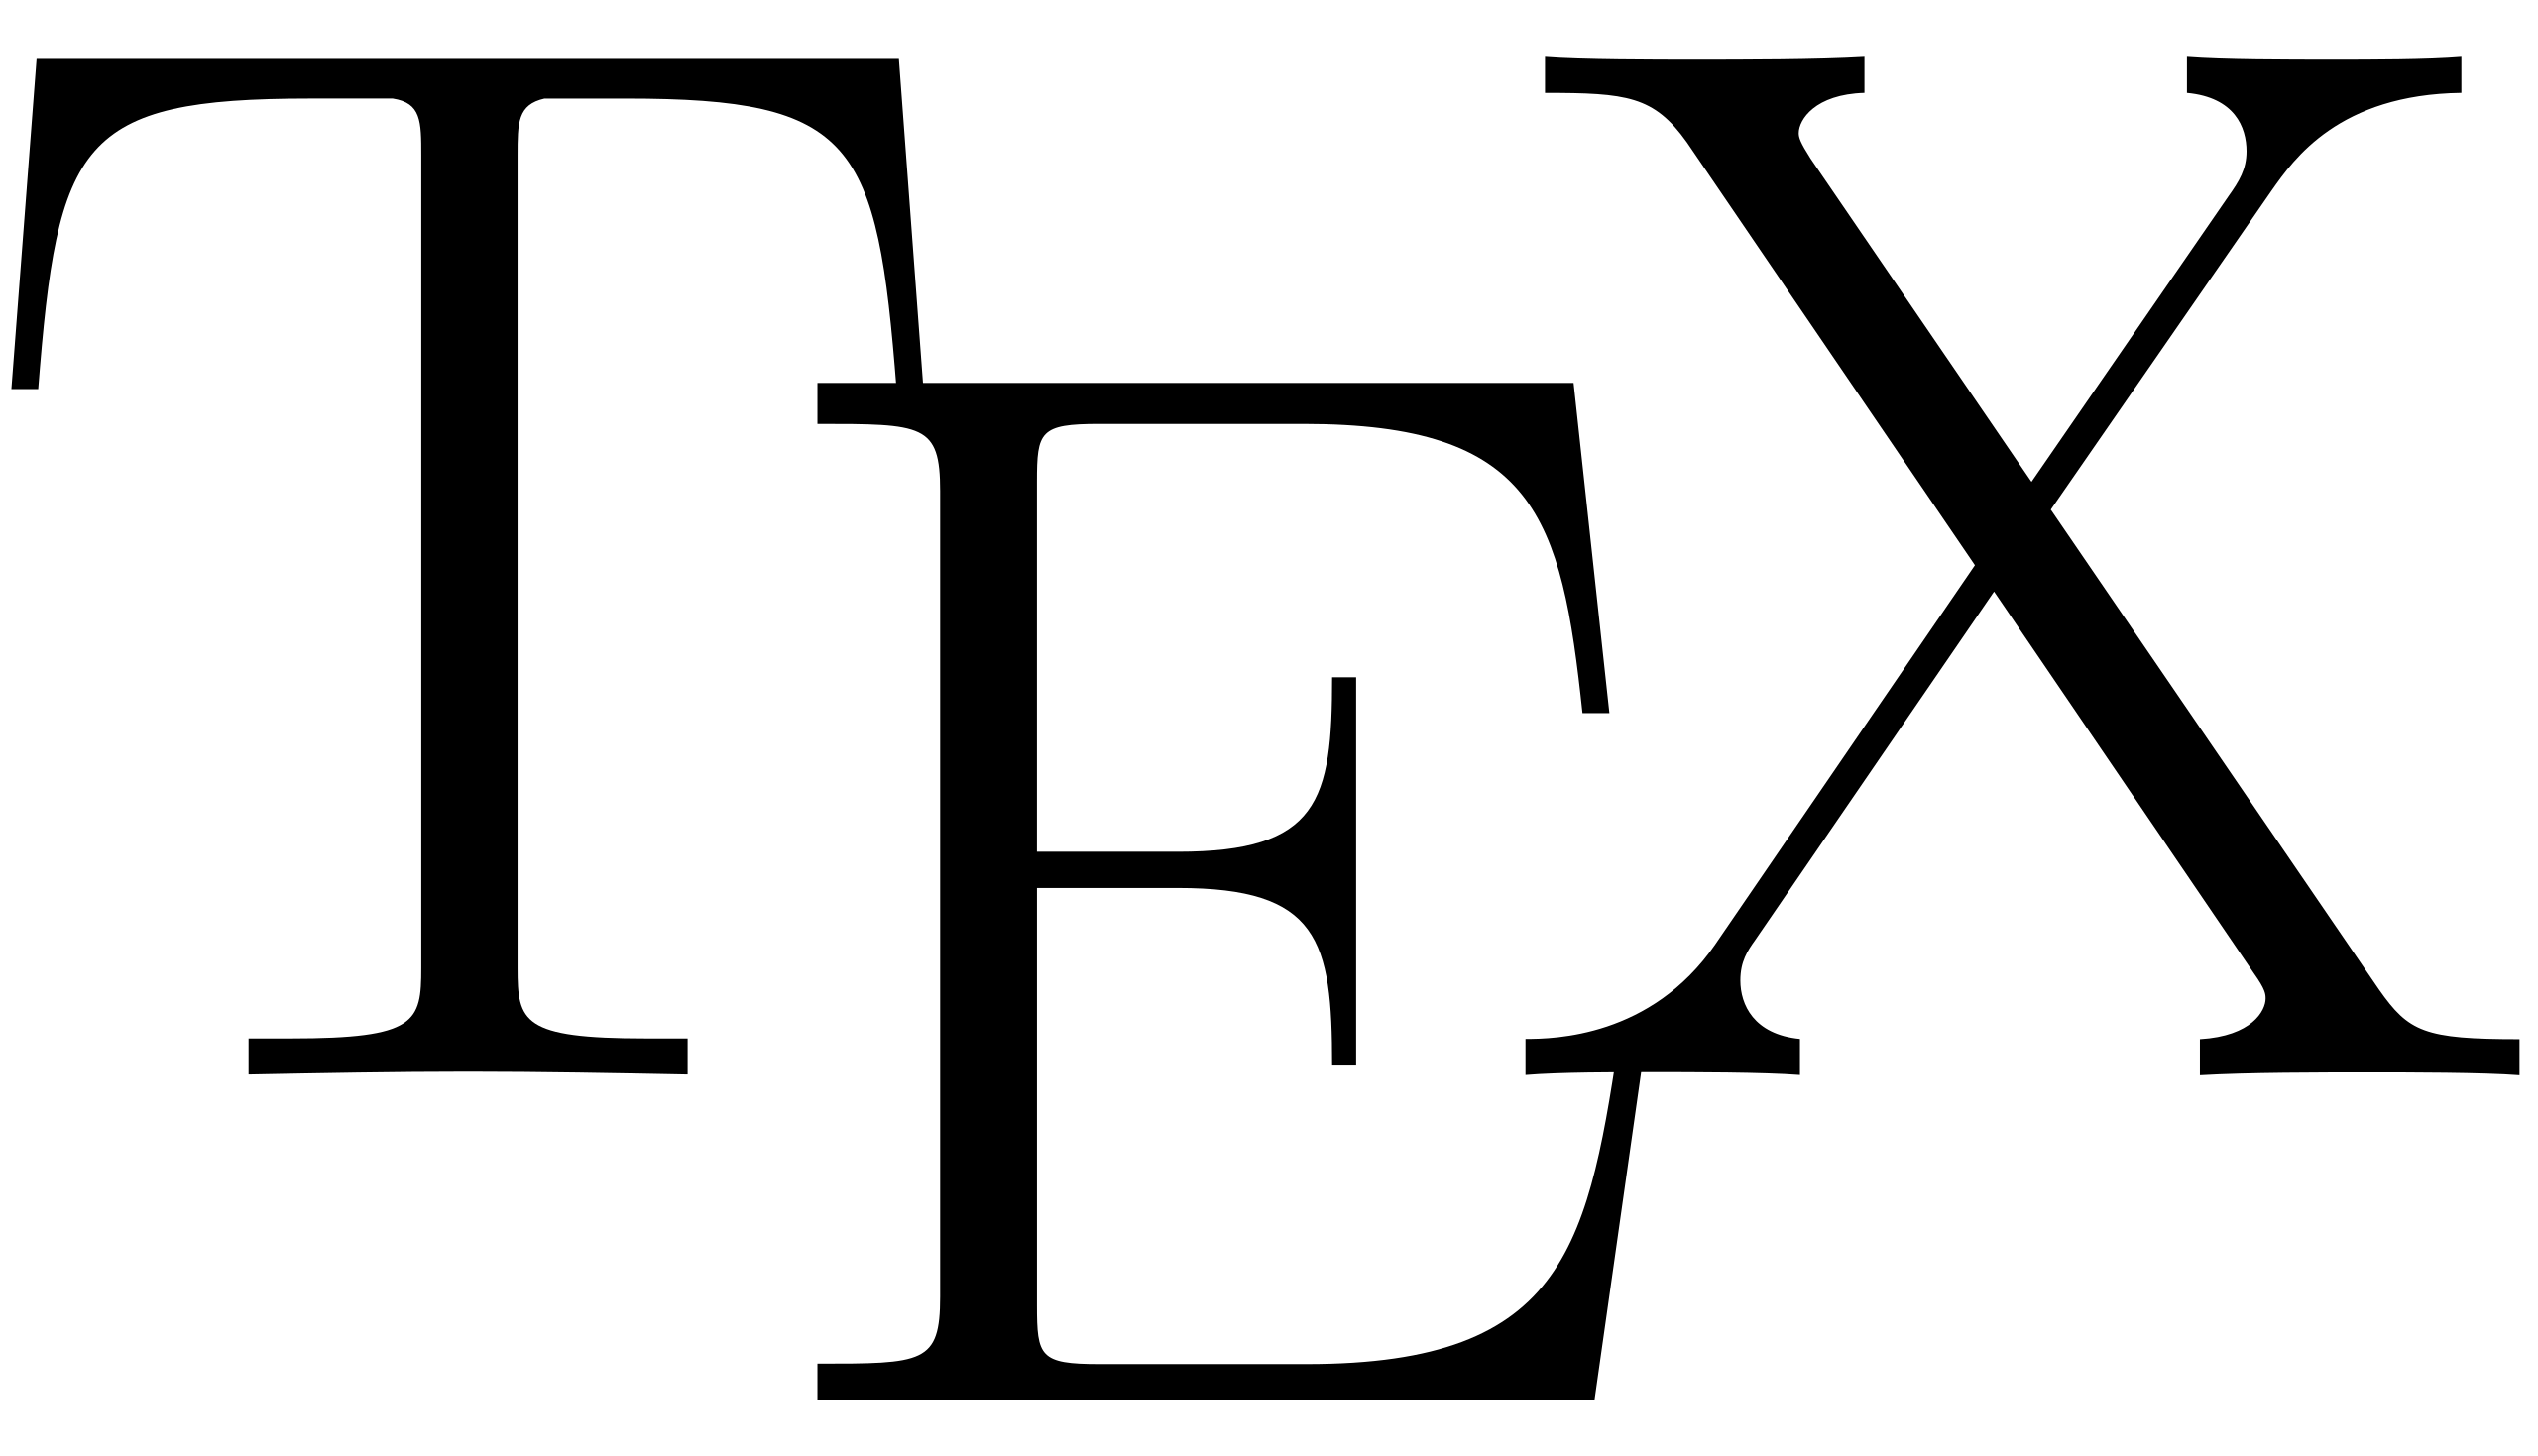
\includegraphics[width=1in]{img/tex_logo.png}
  
  	\TeX{} er eit typesettingssystem for tekstdokument som vart lansert i 1978 av professor Donald Knuth ved Stanford. Motivet bak utviklinga av \TeX{} var at han ønskte eit betre system for å skriva ei serie med bøker som han jobba med.
  	
	%I 1978 lanserte Stanford proffessoren Donald Knuth eit typesettingssystem som han kalte for \TeX{}. 
	
	Formålet med \TeX{} var (og er) at kven som helst med rimelig enkelthet skulle kunne produsera bøker med høg kvalitet (typografisk sett).
	
	Namnet \TeX{} kjem frå gresk \(\tau\epsilon\chi\nu\eta\) som tyder ferdighet eller kunst. Den siste bokstaven i \TeX{}, $\chi$ er ein stor ``chi'', og uttalen av ordet \TeX{} er ``tekh''.
	
\end{frame}

\begin{frame}{\LaTeX}
	
	\includesvg[width=1.5in]{img/latex-project-logo.svg}
	
	\TeX{} kan vera ganske tungvindt å nytta direkte, og gir brukaren litt for mykje fleksibiliet i å styra utforminga av dokumentet. Når ein skriv eit dokument er det normalt ynskjeleg at dokumentet fylgjer ein gitt standard for typografi utan at ein manuelt må passe på dette.
	
	\LaTeX{} er ein utvidelse til \TeX{} i form av ulike makroar som er koda i \TeX{}. Prosjektet for å utvikla \LaTeX{} vart starta av Leslie Lamport på 1980 talet, og den første utgåva vart lansert i 1984. \LaTeX{} har ulike tillegg for å gjera det enklare å utarbeida dokument i henhold til ein gitt standard. Dvs. med ein gitt skrifttype, gitte margar, linjeavstandar og andre parameter som det er naturleg at skal vera konsekvent gjennom heile dokumentet. Ulike malar er tilgjengeleg for ulike dokumenttypar, og det er også mogleg å laga sine eigne malar.
	
\end{frame}


%%% Local Variables:
%%% mode: latex
%%% TeX-master: "../latex-presentation"
%%% End:
